\chapter{Marco de Referencia}

 Desde finales del siglo pasado, los avances tecnológicos en la miniaturización de la electrónica y los componentes mecánicos han allanado el camino para la creación y desarrollo de objetos voladores de pequeñas dimensiones, tales como aviones y helicópteros, los cuales están adquiriendo cada vez más habilidades para realizar vuelos de forma autónoma. Estos dispositivos son popularmente conocidos como drones, un término derivado del inglés \say{abejorros}, y se consideran máquinas voladoras autónomas o semi-autónomas capaces de llevar a cabo misiones de vuelo. En el ámbito internacional, se les conoce como UAVs del ingles \say{Unmanned Aerial Vehicles}, y representan una tecnología compleja cuyo control presenta desafíos, dado que sus características aerodinámicas son similares a las de las aeronaves convencionales \cite{eisenbeiss2004mini}.

El estudio de estos dispositivos despierta un gran interés debido a su versatilidad y capacidad de maniobra, lo que les permite llevar a cabo una amplia gama de tareas en diversas aplicaciones, tales como el uso civil, militar y aeroespacial \cite{nawaz2019applications, shakhatreh2019unmanned, xiaoning2020analysis}. En la figura \ref{fig1_aplicacion_UAV}, se presenta una clasificación detallada de las aplicaciones más importantes de los UAVs.

\begin{figure}[H]
    \centering
    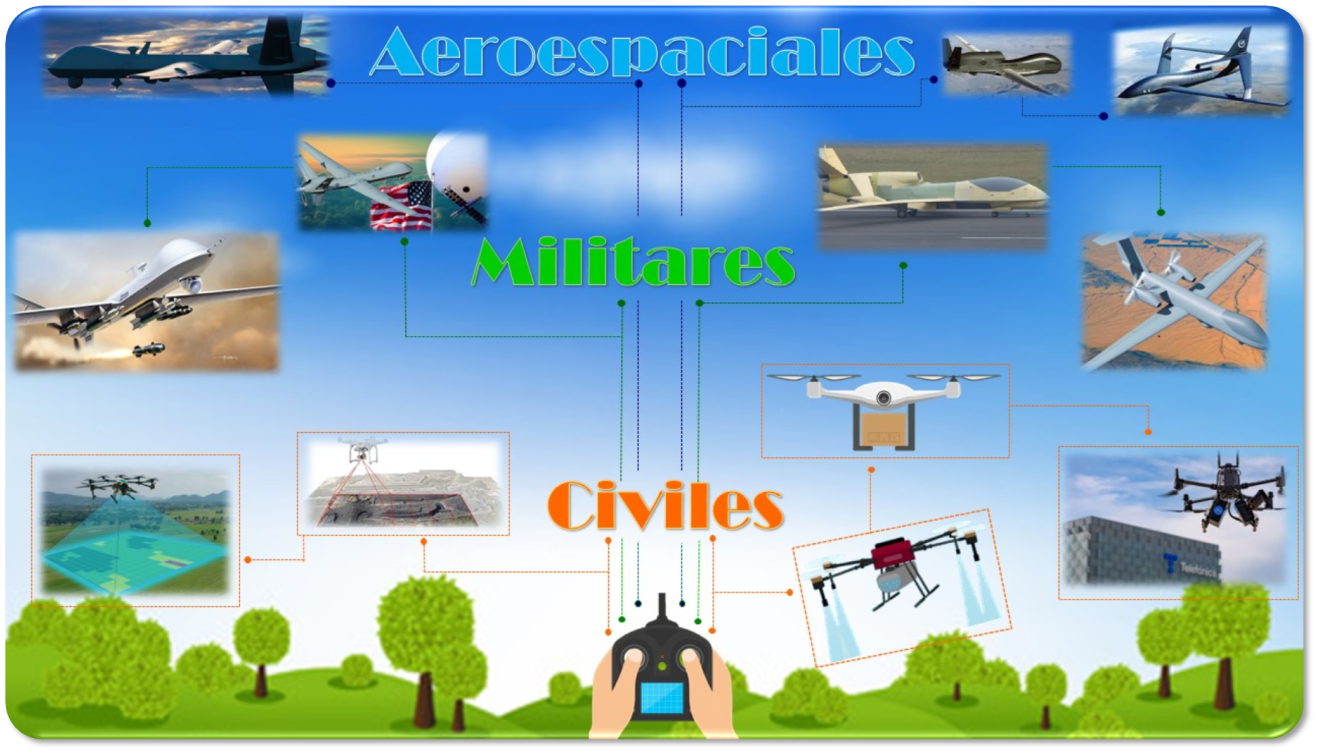
\includegraphics[width=16cm, height=7.5cm]{imagenes/Aplicaciones_UAV.png}
    \caption{Áreas de aplicación UAVS.}
    \label{fig1_aplicacion_UAV}
\end{figure}

\section{Antecedentes.}

Los drones han atraído la atención de la comunidad investigadora que trabaja tanto en el campo militar como en el civil, con una gran cantidad de usos que han sido propuestos por los grupos de investigación, debido a sus características como capacidad y configuraciones, donde el helicóptero de cuatro rotores tiene el mayor número de citas en la literatura de control y ha sido ampliamente investigado para pruebas tanto en interiores como en exteriores . 

\section{Objetivo General}
Desarrollar un sistema web para la gestión de actividades dentro de una farmacia, utilizando una arquitectura y herramientas del entorno de Laravel, para asegurar la trazabilidad de los productos médicos, minimizar los errores de registro manual y proporcionar un soporte analítico para la gestión estratégica del negocio.

\section{Objetivos Específicos}
\begin{enumerate}
\item Identificar las necesidades relacionadas con los procesos de control de una farmacia, mediante una investigación, para la elaboración completa del proyecto.
\item Diseñar la arquitectura de la base de datos e interfaz del sistema, mediante herramientas y tecnologías web, para organizar de mejor manera la información.
\item Implementar módulos de control, con Laravel y MariaDB, para el registro, actualización, salida y existencia de medicamentos.
\item Generar alertas automáticas sobre caducidades próximas y niveles mínimos de existencias, utilizando las herramientas proporcionadas por el framework, para evitar pérdidas.
\item Evaluar el funcionamiento del sistema, mediante pruebas de sus módulos y la generación de reportes estadísticos, para verificar la precisión de los registros y favorecer la toma de decisiones.
\end{enumerate}

\section{Alcance}


\section{Limitaciones del Sistema}
\begin{enumerate}
\item \textbf{Conexión a internet:} Se implementará un sistema accesible desde diferentes dispositivos mediante una conexión de red. Además, se buscará incorporar mecanismos de almacenamiento local o recuperación de información para reducir las interrupciones ocasionadas por fallas de conectividad. El servidor contará con mecanismos de disponibilidad y recuperación ante posibles fallos.
\item \textbf{Control de usuarios:} Se implementará un módulo de autenticación y autorización que permita administrar usuarios mediante roles y permisos específicos. Se contemplarán diferentes niveles de acceso, como administrador y personal encargado del inventario, con el propósito de proteger la información y evitar modificaciones no autorizadas.
\item \textbf{Actualización de información:} Se incorporará un registro de movimientos de inventario que permita controlar las entradas, salidas, devoluciones y ajustes de medicamentos. También se incluirá un historial de movimientos para identificar quién realizó cada operación y cuándo se llevó a cabo, reduciendo los errores de captura y manteniendo actualizada la información.
\item \textbf{Funciones limitadas:} El sistema contará con módulos enfocados en la administración y control de medicamentos, incluyendo registro, edición, consulta, clasificación, control de existencias, fechas de caducidad y generación de reportes. Las funcionalidades adicionales podrán incorporarse posteriormente de acuerdo con las necesidades de la institución.
\item \textbf{Sin integración externa:} Se diseñará una estructura que permita futuras integraciones con proveedores, sistemas de facturación y plataformas externas mediante interfaces de comunicación (API). En la primera versión, la administración de la información se realizará directamente desde el sistema, sin depender de servicios externos.
\item \textbf{Mantenimiento del sistema:} Se establecerá un plan de mantenimiento preventivo y correctivo que contemple actualizaciones, revisión de errores, optimización del funcionamiento y generación periódica de copias de seguridad. Asimismo, se considerarán mecanismos de restauración de datos para garantizar la continuidad y confiabilidad de la información.
\end{enumerate}

\section{Problemática}


\section{Justificación}

